\chapter{Desarrollo}
\thispagestyle{empty}

\section{Descripción del capítulo} \label{sec:\thesection}
En este capitulo se desarrollarán las soluciones propuestas en el capítulo de diseño. Esto implica detallar el proceso realizado, describir los cambios que se debieron hacer en caso de que el planteo inicial no haya funcionado, análisis de resultados, etc. \\
Cada sección será redactada en el orden que se hicieron, debido a que unas partes dependen de otras para poder desarrollarse.

\section{Firmware del updown - Librerías de bajo nivel} \label{sec:\thesection}

\subsection{DigitalIO}
%El desarrollo del módulo de entradas y salidas digitales (DigitalIO) está basado en el capítulo 18 de la hoja de datos del Atmega328p. 

\subsubsection{Manejo del periférico}

Las entradas y salidas digitales del Atmega328p se manejan mediante 3 registros: el DDRn (Data Direction Register n), PORTn (Port n Data Register) y PINn (Port n Input Pins Address). La "n" en los registros se refiere al registro específico a ser accedido, que en el caso de este microcontrolador puede ser B, C o D.\\

Para inicializar un pin como entrada o salida digital primero se elige la dirección del mismo, o sea, si se utilizará como entrada O como salida digital. Para esto se utiliza el registro DDRn, en donde escribir un bit de este registro en 1 significa configurar el pin asociado a este bit como Output (salida) o , mientras que si se escribe en 0 significa configurar al pin como Input (entrada). Para el caso de las entradas se puede optar por habilitar una resistencia pull-up interna del microcontrolador. El pull-up se encuentra deshabilitado por defecto, pero puede ser habilitado escribiendo un 1 en el bit análogo del registro PORTn.
Para escribir el valor de un pin configurado como salida se setea su valor mediante el registro PORTn. Un 1 en un bit de este registro significa poner en HIGH (5 Volts) la salida asociada a ese bit, mientras que un 0 es un estado LOW (0 Volts).\\
La lectura del estado de un pin configurado como entrada se hace a través del registro PINn. Enmascarando un bit específico en el puerto se puede obtener ese valor en particular.

Por ejemplo, si se quiere inicializar el bit 3 del puerto B como entrada con pull-up y el bit 6 del puerto D como entrada en lenguaje C, se tiene:

\begin{lstlisting}[style=CStyle]
	/* --- Configuracion bit 3 puerto B como Input - Pullup --- */
	// Inicializacion del pin
	DDRB &= ~(1 << 3); // Inicializacion como entrada
	PORTB |= (1 << 3); // Habilitacion pullup
	
	// Lectura del estado del pin
	estadoBit3PuertoB = PINB & (1 << 3);
	
	/* --- Configuracion bit 6 puerto D como Output --- */
	// Inicializacion del pin como salida
	DDRD |= (1 << 6); 
	
	// Escritura de un 1 en el pin
	PORTD |= (1 << 6); 
\end{lstlisting}

\subsubsection{Implementación}

Ahora, conocer el bit, puerto y nombres de los registros para cada pin a configurar es muy tedioso. Por lo tanto, para facilitar la lecto-escritura y configuración de los pines se mapearon los bits de los puertos B,C y D a números, como se muestra en la tabla \ref{table:3.1}. El criterio de enumeración fue basado en los pines del Arduino UNO.

\begin{table}[!ht]
	\begin{center}
		\begin{tabular}{|c|c|c|}
			\hline
			\textbf{Puerto} & \textbf{Bit} & \textbf{Numero mapeado} \\
			\hline \hline
			D & 0, 1, 2, 3, 4, 5, 6, 7 & 0, 1, 2, 3, 4, 5, 6, 7 \\
			\hline
			B & 0, 1, 2, 3, 4, 5 & 8, 9, 10, 11, 12, 13 \\
			\hline
			C & 0, 1, 2, 3, 4, 5 & 14, 15, 16, 17, 18, 19\\
			\hline
		\end{tabular}
	\end{center}
	\caption{Mapeo de bits de los puertos a número}
	\label{table:\thetable}
\end{table}

Para acceder al módulo se implementaron 3 funciones, una de inicialización, una de  lectura y otra de  escritura, y 3 definiciones para configurar los pines, entrada, salida y salida con pullup, como se muestra en la figura \ref{fig:3.1}. De esta forma, el ejemplo resuelto mediante registros queda de la siguiente manera:

\begin{lstlisting}[style=CStyle]
	/* --- Configuracion bit 3 puerto B como Input - Pullup --- */
	// Inicializacion del pin como entrada con pullup
	DigitalIO_init(11, DigitalIO_INPUT_PULLUP); // Puerto B bit 3 = 11
	
	// Lectura del estado del pin
	estadoBit3PuertoB = DigitalIO_read(11);
	
	/* --- Configuracion bit 6 puerto D como Output --- */
	// Inicializacion del pin como salida
	DigitalIO_init(6, DigitalIO_OUTPUT); // Puerto D bit 6 = 6
	
	// Escritura de un 1 en el pin
	DigitalIO_write(6, 1);
\end{lstlisting}

\begin{figure}[!ht]
	\centering
	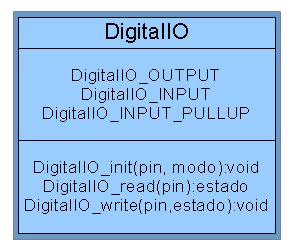
\includegraphics[width=6cm,scale=1]{resources/3_1-moduloDigitalIO.png}
	\caption{Diagrama del módulo DigitalIO}
	\label{fig:\thefigure}
\end{figure}


\subsection{ADC}
%El desarrollo del módulo ADC está basado en el capítulo 28 de la hoja de datos del Atmega328p.

\subsubsection{Manejo del periférico}
El periférico de lectura de entrada analógica del Atmega328p es un ADC por \textit{aproximaciones sucesivas} de 10bits de resolución. Esto quiere decir que la conversión se realiza a una frecuencia determinada, y con una tensión de referencia dada. Además, este microcontrolador cuenta con 1 solo módulo de ADC y 8 canales analógicos, por lo que el usuario debe elegir a qué canal irá el resultado de la conversión mediante un multiplexor de entradas. El diagrama completo del sistema de conversión se encuentra en la figura 28.1 del datasheet del atmega328p.

La incialización del periférico se logra mediante los registros ADMUX (ADC Multiplexer Selection Register) y ADCSRA (ADC Control and Status Register). Con el primero se selecciona la tensión de referencia, mientras que con el segundo se habilita el periférico y se selecciona la frecuencia de la conversión mediante la selección de un preescalador. Por ejemplo, si se desea utilizar como referencia de tensión la Vcc del micro (5V) y se quiere una frecuencia de 125KHz el código, en lenguaje C, sería:
\begin{lstlisting}[style=CStyle]
	/* Selecciono Vref = Vcc */
	ADMUX = (1 << REFS0);

	/* Habilitacion del adc y seteo del prescaler a 128 => f_adc = 125KHz */
	ADCSRA = (1 << ADEN) | (1 << ADPS2) | (1 << ADPS1) | (1 << ADPS0); 
\end{lstlisting}
Cabe aclarar que REFS0 es el bit asociado a la selección de Vref = Vcc. Es el 6to bit del registro ADMUX, por lo que REFS0 = 6. Similarmente, ADEN = 7, ADPS2 = 2, ADPS1 = 1 y ADPS0 = 0.

Luego, para la lectura del valor analógico se debe:
\begin{enumerate}
	\item Seleccionar el canal mediante el multiplexor de entradas con el registro ADMUX. Los 3 bits menos significativos, llamados MUX0/1/2, de este registro permiten seleccionar los canales: si MUX[2:0] = 000 => selecciono el canal 0, si es igual a 001 selecciono el canal 1, y así hasta llegar a 111 para el canal 7.

	\item Dar comienzo a la conversión poniendo un 1 en bit 6 (llamado ADSC) del registro ADCSRA.
	\item Esperar a que termine la conversión. Cuando la conversión termina ADSC, que había sido seteado en 1, pasa a valer 0.
	\item Recuperar el resultado leyendo el registro ADC.
\end{enumerate}

El ejemplo de lectura del canal 2, en lenguaje C, sería:
\begin{lstlisting}[style=CStyle]
	/* --- Lectura de un dato del canal 2 --- */
	// Seleccion del canal que se desea leer conservando el resto de los valores del registro
	ADMUX = (ADMUX & 0b11111000)| 2; // 2 debido al canal a ser leido
	
	// Inicio de conversion
	ADCSRA |= (1<<ADSC);
	
	// Espera del fin de la conversion
	while(ADCSRA & (1<<ADSC));
	
	// Lectura del valor resultante de la conversion
	valorCanal2 = ADC;
\end{lstlisting}

\subsubsection{Implementación}

Para acceder al módulo se implementaron 2 funciones, una de inicialización y una de lectura, como se muestra en la figura \ref{fig:3.2}. De esta forma, los ejemplos resueltos mediante registros quedan de la siguiente manera:

\begin{lstlisting}[style=CStyle]
	/* --- Inicializacion del periferico --- */
	ADC_init(); 
	
	/* --- Lectura del canal 2 --- */
	valorCanal2 = ADC_read(2);
\end{lstlisting}

\begin{figure}[!ht]
	\centering
	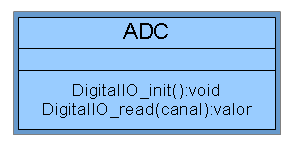
\includegraphics[width=6cm,scale=1]{resources/3_2-moduloADC.png}
	\caption{Diagrama del módulo ADC}
	\label{fig:\thefigure}
\end{figure}

\subsection{PWM}
%El desarrollo del módulo PWM está basado en el capítulo 20 de la hoja de datos del Atmega328p.
\subsubsection{Frecuencia}
La frecuencia del PWM a generar será de 25KHz, ya que:
\begin{itemize}
	\item Es lo suficientemente rápida como para que el motor integre la señal y la tome como continua.
	\item Al encontrarse por encima de 20KHz, que es el tope del rango audible, no provoca ruidos indeseados.
	\item Es soportada por los mosfets utilizados en el puente H (NTD3055L104).
\end{itemize}

\subsubsection{Manejo del periférico}
En el Atmega328p no existe un periférico exclusivo para generación de PWM. Por lo tanto, se generará con el periférico Timer del microcontrolador. De los Timers que tiene este microcontrolador, el más potente para generación de PWM es el Timer1, puesto que cuenta con un modo de generación de PWM de fase correcta. Este modo es preferible por sobre el modo de pwm soportado por los otros 2 timers (0 y 2) ya que no provoca corrimientos de fase durante la variación del ancho del pulso, efecto que hay que evitar en el control de motores.

La generación de PWM en modo fase correcta se hace a través de la comparación de un contador (TCNT1) con un valor definido por el usuario (OCR1A). La señal de PWM sale por una salida digital especial llamada OCR1A, y la forma de la señal depende del tipo de comparación. Si el tipo de comparación es no-invertida, OCR1 vale 1 si el TCNT1 es menor a ICR1, y 0 en caso contrario. De esta manera, se puede ajustar el ciclo de trabajo al variar el valor de ICR1. En la figura \ref{fig:3.3} se muestra la señal en OC1A si el timer se encuentra en modo fase correcta con comparación tipo no-invertida, al variar el valor de OCR1A. A medida que este valor sube también lo hace el ciclo de trabajo. La configuración de estos modos de trabajo se hace a través del registro TCCR1A.

\begin{figure}[!ht]
	\centering
	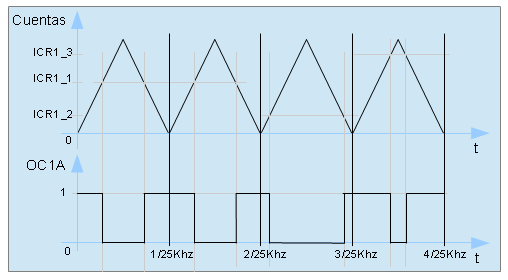
\includegraphics[width=15cm,scale=1]{resources/3_3-generacionPWM.png}
	\caption{Ejemplo variación ciclo de trabajo al cambiar ICR1}
	\label{fig:\thefigure}
\end{figure}

La frecuencia de la señal se puede elegir mediante el registro ICR1. Su valor depende de la frecuencia del microcontrolador (\(f_{cpu}\)), de la frecuencia objetivo (\(f_{pwm}\)) y de un preescalador (N) seleccionable mediante el registro TCCR1B, como se puede ver en la ecuación \ref{eq:3.1}. Para este proyecto el atmega328p trabaja a \(f_{cpu} = 16Mhz\), y la frecuencia objetivo es \(f_{pwm} = 25Khz\), por lo que tomando un preescalador de N=1 se tiene que ICR1 vale exactamente 320.

\begin{equation} \label{eq:\theequation}
	ICR1 = \frac{f_{cpu}}{2.N.f_{pwm}}
\end{equation}



A continuación se presenta un ejemplo de incialización del periférico y selección del ciclo de trabajo, en lenguaje C: 
\begin{lstlisting}[style=CStyle]
	/* --- Inicializacion del periferico --- */
	// Inicializacion del pin asociado a OC1A como salida, que es el 9 (puerto B bit 1).
	DigitalIO_init(9,OUTPUT);
	
	// Configuracion para pwm de fase correcta
	TCCR1A |= (1 << WGM11)|(0 << WGM10); TCCR1B |= (1 << WGM13)|(0 << WGM12);
	
	// Configuracion para tipo de comparacion no-invertida
	TCCR1A |= (1 << COM1A1)|(0 << COM1A0)|(1 << COM1B1)|(0 << COM1B0);
	
	// Configuracion para prescalador = 1
	TCCR1B |= (0 << CS12) | (0 << CS11) | (1 << CS10);
	
	// Configuracion para frecuencia de 25KHz
	ICR1 = 320;
	
	/* --- Seleccion de ciclo de trabajo --- */
	// Ciclo de trabajo de x%: ICR1*x/100. Para 50% se tiene
	OCR1A = 160;
\end{lstlisting}

\subsubsection{Implementación}

Para acceder al módulo se implementaron 2 funciones, una de inicialización y una de escritura, como se muestra en la figura \ref{fig:3.4}. De esta forma, el ejemplo resuelto mediante registros queda de la siguiente manera:

\begin{lstlisting}[style=CStyle]
	/* --- Inicializacion del periferico --- */
	// Inicializacion del pin asociado a OC1A como salida, que es el 9 (puerto B bit 1).
	PWM_init();
	
	/* --- Seleccion de ciclo de trabajo --- */
	PWM_write(50); // ciclo de trabajo a 50%
\end{lstlisting}


\begin{figure}[!ht]
	\centering
	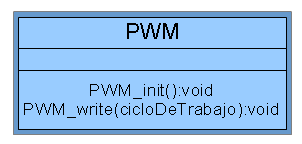
\includegraphics[width=6cm,scale=1]{resources/3_4-moduloPWM.png}
	\caption{Diagrama del módulo PWM}
	\label{fig:\thefigure}
\end{figure}

\subsection{EXINT}
%El desarrollo del módulo de interrupciones externas (EXINT) está basado en el capítulo 17 y 18 de la hoja de datos del Atmega328p.
\subsubsection{Manejo del periférico}
En el atmega328p hay 2 tipos de interrupciones externas:
\begin{itemize} 
	\item Las EXINT, que pueden ser configuradas para que se accionan por cualquier tipo de cambio en un pin (flanco ascendente, descendente y ambos), pero que solo están disponibles en 2 pines.
	\item y las PCINT que siempre se activan con un cambio en el pin (no se puede elegir como en las EXINT), pero que están disponibles para la mayoría de los pines del microcontrolador.
\end{itemize}

Para inicializar las EXINT simplemente se selecciona el tipo de disparo en el registro EICRA, se habilita la entrada digital correspondiente, y habilita la interrupción en el registro EIMSK.\\
Para las PCINT simplemente se habilita la entrada digital correspondiente y habilita la interrupción en el registro PCICR.\\

\subsubsection{Implementación}
Para acceder al módulo se implementaron 2 funciones de inicialización, una para EXINT y otra para PCINT, como se muestra en la figura \ref{fig:3.5}.

Ambos 2 periféricos generan interrupciónes, por lo que al ocurrir el evento disparador se ejecutará la ISR correspondiente. Por este motivo durante la inicialización de una EXINT o PCINT se deberá indicar la función a ejecutar durante la ISR mediante un puntero a función, implementado la siguiente linea en el .h:
\begin{lstlisting}[style=CStyle]
/* --- Inicializacion del periferico --- */
typedef void (*voidFunctionPointer_t)(void);
\end{lstlisting}

Este nuevo tipo de dato es simplemente un parámetro en las funciones de incialización en donde el usuario puede decidir qué se ejecuta durante la interrupción.

\begin{figure}[!ht]
	\centering
	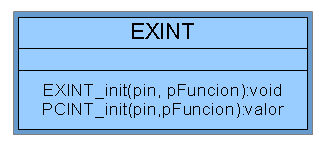
\includegraphics[width=8cm,scale=1]{resources/3_5-moduloEXINT.png}
	\caption{Diagrama del módulo EXINT}
	\label{fig:\thefigure}
\end{figure}


\subsection{UART}
%El desarrollo del módulo UART está basado en el capítulo 24 de la hoja de datos del Atmega328p.
\subsubsection{Manejo del periférico}
El Atmega328p tiene un periférico de UART bastante estándar, en donde se puede configurar su tasa de transmisión (baudrate), modo de operación y formato de trama. Esto se logra por medio de los registros UBRR0, UCSR0A, UCSR0B y UCSR0C.

UBRR0, que se separa en UBRR0H u UBRR0L, sus partes alta y baja respectivamente, de 8 bits cada una, se utiliza para configurar el baudrate. La ecuación \ref{eq:3,2} sirve para obtener el valor de UBRR0, en donde el 16 pasa a ser 8 si el bit U2X0 en el registro UCSR0A está seteado.

\begin{equation} \label{eq:\theequation}
	UBRR0 = \frac{f_{clk}}{(16.BAUD)} - 1
\end{equation}

Como DMX trabaja a una tasa de 250KHz y la frecuencia del microcontrolador es de 16MHz tenemos que UBRR0 = 3, o sea que UBRR0L = 3 y UBRR0H = 0. \\
Mediante el registro UCSR0B se habilita o deshabilita la transmision y recepción de datos. Como los esclavos DMX solo reciben datos, solo hace falta habilitar la recepción, lo cual se logra seteando el bit RXEN0 de este registro. También se pueden habilitar las interrupciones por recepción poniendo en 1 el bit RXCIE0, lo cual es necesario en esta aplicación debido a que durante la interrupción se tiene que analizar la trama DMX. Al igual que para el módulo EXINT, aquí también se utilizará el tipo de dato voidFunctionPointer\_t para que el módulo que llame a este pueda indicar qué función quiere ejecutar durante las interrupciones de recepción.\\
Finalmente, el registro UCSR0C permite configurar el modo (sincrónico o asincrónico) y el formato de la trama. DMX trabaja en modo asincrónico y con formato de trama 8N2.

En cuanto a la recepción, los datos que llegan por el puerto serie se almacenan en el registro UDR0. Para leerlo se verifica si el bit RXC0 en el registro UCSR0A se encuentra en 1, ya que este bit indica si existen datos no leidos en el buffer de recepción.

A continuación se presenta un ejemplo de incialización y lectura de datos del periférico, , en lenguaje C: 

\begin{lstlisting}[style=CStyle]
	/* --- Inicializacion del periferico --- */
	// Configuracion de tasa = 250KHz
	UBRR0H = 0;
	UBRR0L = 3;
	UCSR0A = (0<<U2X0);
	
	//Habilitacion de Rx y su interrupcion
	UCSR0B = (1<<RXEN0)|(0<<TXEN0)|(1<<RXCIE0); 
	
	//Seleccion de modo asincronico, con formato de trama 8N2
	UCSR0C = (1<<USBS0)|(1<<UCSZ01)|(1<<UCSZ00); 

	/* --- Lectura de un dato --- */
	// Se espera a que un dato sea recibido
	while( !(UCSR0A & (1<<RXC0)) ); 
	
	// Se saca el dato del buffer de recepcion
	datoRecibido =  UDR0;
\end{lstlisting}


\subsubsection{Implementación}
Para acceder al módulo se implementaron 2 funciones, una de inicialización y otra de lectura, como se muestra en la figura \ref{fig:3.6}. De esta forma, el ejemplo resuelto mediante registros queda de la siguiente manera:

\begin{lstlisting}[style=CStyle]
	/* --- Inicializacion del periferico --- */
	UART_init(funcion); 
	// "funcion" es la rutina a ejecutar durante la interrupcion
	
	/* --- Lectura de un dato --- */
	datoRecibido =  UART_read();
\end{lstlisting}

\begin{figure}[!ht]
	\centering
	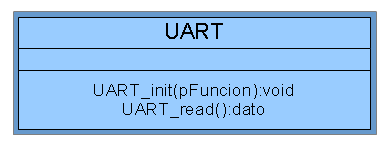
\includegraphics[width=8cm,scale=1]{resources/3_6-moduloUART.png}
	\caption{Diagrama del módulo UART}
	\label{fig:\thefigure}
\end{figure}

\subsection{Tick}
%El desarrollo del módulo Tick está basado en el capítulo 22 de la hoja de datos del Atmega328p
\subsubsection{Frecuencia}
La base de tiempo será de 1ms, equivalente a una frecuencia de 1KHz, ya que si bien la mayoría de las acciones del equipo serán lentas, la actualización del controlador probablemente será del orden de los milisegundos. En caso de necesitarse otra base de tiempo, más chica o más grande, se modificará este valor.

\subsubsection{Manejo del periférico}
Para implementar una base de tiempo como es el módulo Tick es necesario un Timer. El Atmega328p cuenta con 3 timers, de los cuales 1 (el timer 1) ya fue utilizado para el módulo PWM. Los restantes son el 0 y el 2, y ambos pueden generar una señal de 1KHz sin problemas y con mínimo error, por lo que se utilizará el Timer2.

Para generar la base de tiempo se utilizará el modo de comparación (CTC) del timer, seleccionable mediante el registro TCCR2A. En este modo un contador (TCNT2) aumenta hasta igualar un valor definido por el usuario (OCR2A). Cuando esto sucede se reinicia la cuenta y se genera una interrupción si el bit OCIE2A del registro TIMSK2 se encuentra en 1.\\
La frecuencia se configura mediante los registros TCCR2B (seteo del prescalador) y OCR2A, siguiendo la ecuación \ref{eq:3.3}. Como la frecuencia deseada es \(f_{tick} = 1KHz\) y la del microcontrolador es \(f_{cpu} = 16MHz\), con un N = 128 se obtiene que OCR2A = 124.

\begin{equation} \label{eq:\theequation}
OCR2A = \frac{f_{cpu}}{N.f_{tick}}
\end{equation}

A continuación se presenta un ejemplo de inicialización del periférico con una frecuencia de 1KHz e interrupción habilitada, en lenguaje C.

\begin{lstlisting}[style=CStyle]
	/* --- Inicializacion del periferico --- */
	// Configuracion para el modo CTC
	TCCR2A |= (1 << WGM21);
	
	// Seteo de la frecuencia a 1KHz
	TCCR2B |= (1 << CS22) | (0 << CS21) | (1 << CS20); // N = 128
	OCR2A = 124;
	
	// Habilitacion de la interrupcion
	TIMSK2 = (1 << OCIE2A);
\end{lstlisting}

\subsubsection{Implementación}

Durante la interrupción que se genera cuando TCNT2 iguala a OCR2A se incrementa la base de tiempo, contando cada milisegundo que transcurra. Además, con el objetivo de poder implementar un \textit{planificador de tareas} en la capa de aplicación se podrá elegir ejecutar una función durante la interrupción.

Para acceder al módulo se implementaron 2 funciones, una de inicialización y otra de lectura, como se muestra en la figura \ref{fig:3.7}.

\begin{figure}[!ht]
	\centering
	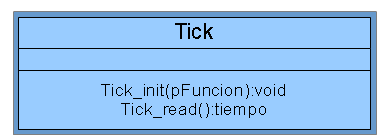
\includegraphics[width=8cm,scale=1]{resources/3_7-moduloTick.png}
	\caption{Diagrama del módulo Tick}
	\label{fig:\thefigure}
\end{figure}

\subsection{SUART}
%El desarrollo del módulo SUART está basado en el capítulo 19 de la hoja de datos del Atmega328p.
\subsubsection{Análisis}
La idea de una UART por software (SUART) es poder establecer una comunicación serie utilizando 2 pines cualesquiera del microcontrolador, sin hardware adicional como se tiene en el periférico UART. Hay muchas formas de lograr esto, desde polling periódico hasta el uso de múltiples interrupciones para lograr la comunicación con el menor consumo de CPU posible. 

Este módulo implementará la SUART haciendo uso del timer 0, que es el único que queda disponible (El 1 genera PWM y el 2 la base de tiempo). La función del timer será generar interrupciones cada cierto tiempo y verificar el estado de los pines asociados a Rx (entrada) y Tx (salida). 

Un canal serie se encuentra en High por defecto, si no se envían datos. Luego se envía el bit de start (Low), los datos, el bit de paridad si lo hay, y el/los bit de stop (High). En nuestro caso el formato de trama es 8N1 por lo que un mensaje transmitido o recibido será un bit en 0, los 8 bits de datos, y un bit en 1.Teniendo en cuenta esto, se tiene que:

Para la salida de datos simplemente se cambia el estado del pin de Tx según el formato de la trama y del dato a enviar. Por ejemplo, si se quiere enviar una 'a', que equivale a 01100001, con una trama 8N1, se enviará 0 (bit de start), luego del bit menos al más significativo del dato (empiezo con 1, luego envío el 0.. etc) y finalmente 1 (bit de stop).

Para la entrada de datos lo que se hace es muestrear el canal cada cierto tiempo e ir reconstruyendo el dato. Por defecto el canal se encuentra en 1, por lo que empiezo a guardar bits cuando un 0 es recibido. Luego verifico que después del dato esté el bit de stop (si no hay paridad).

\textcolor{FIXME}{FALTA DESARROLLAR Y REESTRUCTURAR BIEN TODO. TAMBIéN TENES QUE HACER UN DIAGRAMA DE FLUJO PARA TX Y PARA RX}

La comunicación serie tendrá las siguientes características: formato de trama 8N1 (8 bit de datos, sin paridad, 1 bit de stop) y tasa de transmisión de 9600baudios. Se elije una tasa chica ya que las interrupciones del timer ocurrirán por lo menos 2 veces más rápido que esta tasa, y con interrupciones como la de DMX que tienen una frecuencia de 250Khz los recursos deben cuidarse.

\subsubsection{Implementación}





\subsection{Diagrama de módulos de la librería de bajo nivel}


\section{Controlador} \label{sec:\thesection}

\subsection{Relación entre cuentas de encoder y distancia}
Como se mencionó en la sección \ref{sec:2.3}, subsección 3, 

\subsection{Determinación de la velocidad máxima}

\subsection{Obtención del período de muestreo}
Como se mencionó en la sección \ref{sec:2.3}, subsección 3, 

\subsection{Obtención del modelo de la planta}

\subsection{Obtención del controlador}

\subsection{Ajuste del controlador}


\section{Dipswitch} \label{sec:\thesection}

\section{Firmware del updown - Librerías de alto nivel} \label{sec:\thesection}

\subsection{Encoder}

Por como están conectado los componentes electrónicos en la placa de control, el encoder del motor está asociado a las EXINT y el encoder del disco a las PCINT.

\subsection{Diagrama de módulos de la librería de alto nivel}

\section{Firmware del updown - Función principal} \label{sec:\thesection}


